\documentclass{beamer}
\mode<presentation>
{
  \usetheme{myulm}
  \setbeamercovered{transparent}
  \setbeamertemplate{navigation symbols}{} % no navigation bar
  \setbeamersize{sidebar width left=1.17cm}
}

\usepackage[ngerman]{babel}
\usepackage[utf8]{inputenc}
\usepackage{amsmath,amssymb,amsfonts}
\usepackage{times}
\usepackage{graphicx}
\usepackage{fancyvrb}
\usepackage{array}
\usepackage{colortbl}

% Anfang der Titelfolie
% Anpassung von: Titel, Untertitel, Autor, Datum und Institut

\title{Kanonische Transformationen und die Hamilton-Jacobi-Gleichung}
\subtitle{Seminar I für Computationals Science and Engineering bei Prof. Lebiedz}
\author{Alexander Dürr und Anton Hügel}
\newcommand{\presdatum}{8. Februar 2018} % alternativ zu \today: Eingabe eines festen Datums
\institute
{\\Universität Ulm, Institut für Numerische Mathematik}
%Ende der Titelfolie

% Anfang der Kopfzeile der Folien
% Anpassung von: Zwischentitel, Leitthema oder Name
% Das Datum wird oben geändert: unter \presdatum{}!

\newcommand{\zwischentitel}{Zwischentitel}
\newcommand{\leitthema}{Lanczos Kap. 7 und 8}
% Ende der Kopfzeile

% Anfang der Folien
\begin{document}
\hspace*{-1.49cm}
\frame[plain]{\titlepage}

% Das Inhaltsverzeichnis
\hspace*{-0.7cm}
\begin{frame}
  \frametitle{Inhaltsverzeichnis}
  \tableofcontents
\end{frame}


\section{Bekanntes: Die kanonischen Gleichungen}

\section{Kanonische Transformationen}
    \begin{frame}
    \frametitle{Gesucht: Lösung der kanonischen Gleichungen}
    
    \begin{align*}
        \dot{q}_k &= \frac{\partial H}{\partial p_k} \\
        \dot{p}_k &= -\frac{\partial H}{\partial q_k}
    \end{align*}
    
    
\end{frame}

    \subsection{Lösung mechanischer Probleme mittels Koordinatentranformation}
    \begin{frame}
    \frametitle{Ausweg: Koordinatentransformation}
    
    Gesucht wird ein Koordinatensystem, indem die kanonischen Gleichungen direkt gelöst werden können.
    
    \begin{figure}
        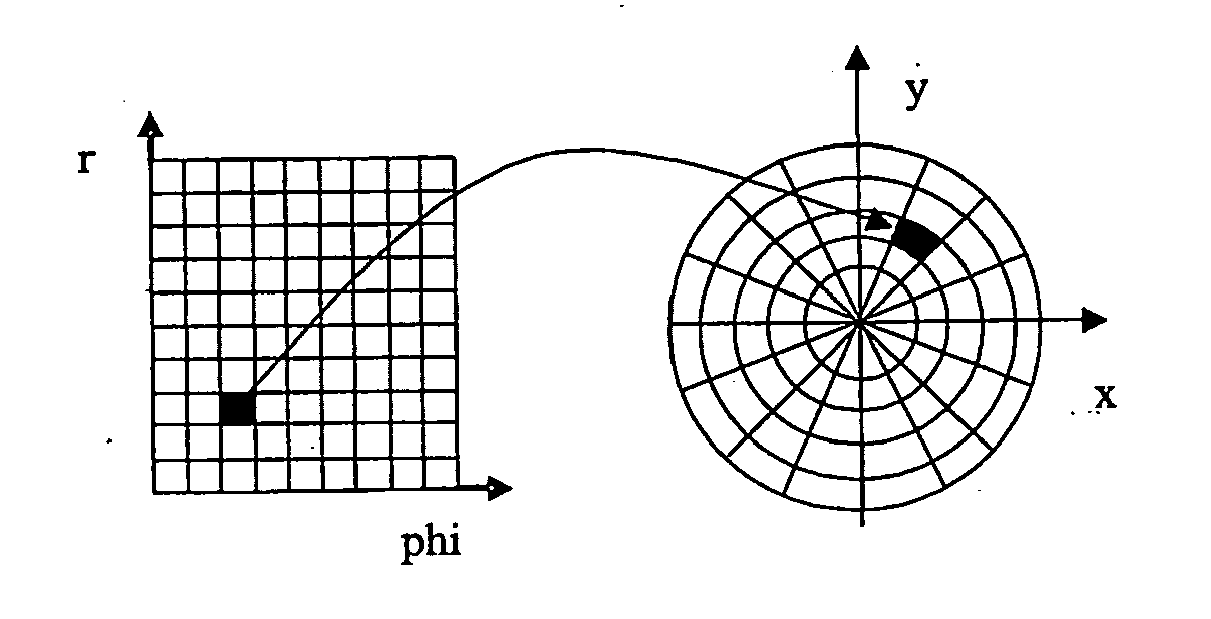
\includegraphics[scale=0.2]{images/koordtrans.png}
    \end{figure}
    
    
\end{frame}

\begin{frame}
    \frametitle{Ausweg: Koordinatentransformation}
    
    \textbf{Wichtig:} Lösungen müssen erhalten bleiben.\\
    D.h. wir brauchen Transformationen, gegenüber derer die kanonischen Gleichungen invariant sind. \\
    \vspace{5mm}    
    Solche Transformationen werden \emph{kanonische Transformationen} genannt.
    
    \begin{figure}
        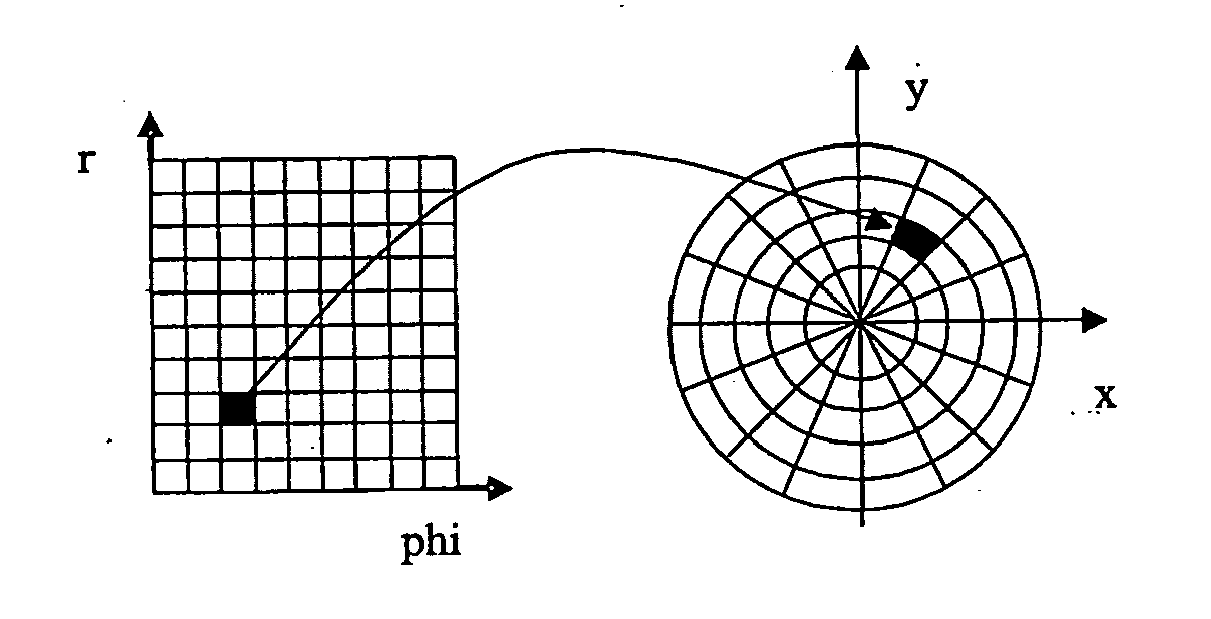
\includegraphics[scale=0.2]{images/koordtrans.png}
    \end{figure}
    
    
\end{frame}
    
    \subsection{Die Langrange'sche Punkttransformation}
    \begin{frame}
    \frametitle{Punkttransformation}
    
    Alte Koordinaten: $p_k, q_k$ \\
    Neue Koordinaten: $P_k, Q_k$
    
    Punkttransformationen haben die Form
    
    \begin{align*}
    q_1 &= f_1(Q_1,\ldots,Q_n) \\
        &\quad\vdots \\
    q_n &= f_n(Q_1,\ldots,Q_n)    
    \end{align*}
    
\end{frame}


    
    \subsection{Die allgemeine kanonische Transformation}
    \begin{frame}
    Die Invarianz von    
    \begin{displaymath}
            \sum_{i=1}^n p_i \delta q_i = \sum_{i=1}^n P_i \delta Q_i
    \end{displaymath}
    ist nicht notwendig. \\
    
    Allgemeinerer Ansatz:
    \begin{displaymath}
    \sum_{i=1}^n p_i \delta q_i = \sum_{i=1}^n P_i \delta Q_i + \delta S
    \end{displaymath}

\end{frame}

\begin{frame}

    Das kanonische Integral sieht nun folgendermaßen aus:
    
    \begin{align*}
    A &= \int_{t_1}^{t_2} \left( \sum_{i=1}^n p_i dq_i - H dt \right) \\
      &= \int_{t_1}^{t_2} \left( \sum_{i=1}^n P_i dQ_i - H dt \right)  +  \underbrace{\int_{t_1}^{t_2} dS}_{=\text{const.}}
    \end{align*}
    
    $\Longrightarrow$  Kannonische Gleichungen invariant unter dieser Transformation.
    
\end{frame}

\begin{frame}
    \frametitle{Allgemeine kanonische Transformation}
    
    
    \begin{displaymath}
        \sum_{i=1}^{n} (p_i \delta q_i - P_i \delta Q_i) = \delta S
    \end{displaymath}
    
    \begin{center} mit der generierenden Funktion $S = S(q_1,\ldots,q_n;Q_1,\ldots,Q_n)$ \end{center}
    
\end{frame}
    
    \subsection{Die bilineare Differentialform}
    \begin{frame}
    \frametitle{Die blineare Differenzialform}
    \begin{itemize}
        \item Jeder Transformation lässt bestimmte Größen unverändert
        \item Diese Invarianten bestimmen Eigenschaften der Transformation
        \item Für kanonische Transformation hatten wir zunächst $\sum p_i \delta q_i$
        \item Dann fanden wir die allgemeinere Bedingung     
                \begin{displaymath}
                \sum_{i=1}^{n} (p_i \delta q_i - P_i \delta Q_i) = \delta S
                \end{displaymath}
              Welcher Invarianten entspricht diese Bedingung?
    \end{itemize}
\end{frame}

\begin{frame}
   
        \begin{displaymath}
        \sum_{i=1}^{n} p_i \delta q_i - \sum_{i=1}^{n} P_i \delta Q_i = \delta S
        \end{displaymath}
        
        $\longrightarrow$ Erinnert an die Arbeit in einem monogenen (monogenic) System.\\
        \vspace{3mm}
        \emph{Masseteilchen wird auf beliebigem geschlossenen Pfad bewegt.\
              Ist die verrichtete Arbeit Null, wenn man wieder am Ausgangspunkt ankommt, so nennt man das System monogen.}
            
      \begin{center} 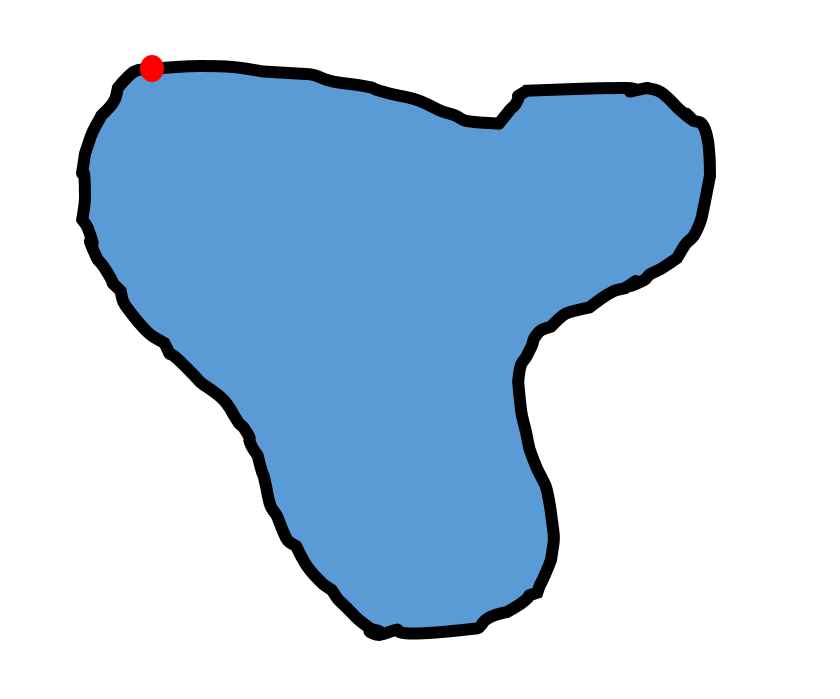
\includegraphics[scale=0.15]{images/monogenicSys}  \end{center}  
        
        

\end{frame}

\begin{frame}
    Integration von
    \begin{displaymath}
    \sum_{i=1}^{n} p_i d q_i - \sum_{i=1}^{n} P_i d Q_i = d S
    \end{displaymath}
    entlang einer geschlossenen Kurve ergibt.
   \begin{displaymath}
   \oint \sum_{i=1}^{n} p_i d q_i - \oint \sum_{i=1}^{n} P_i d Q_i = 0
   \end{displaymath}
    \begin{center} 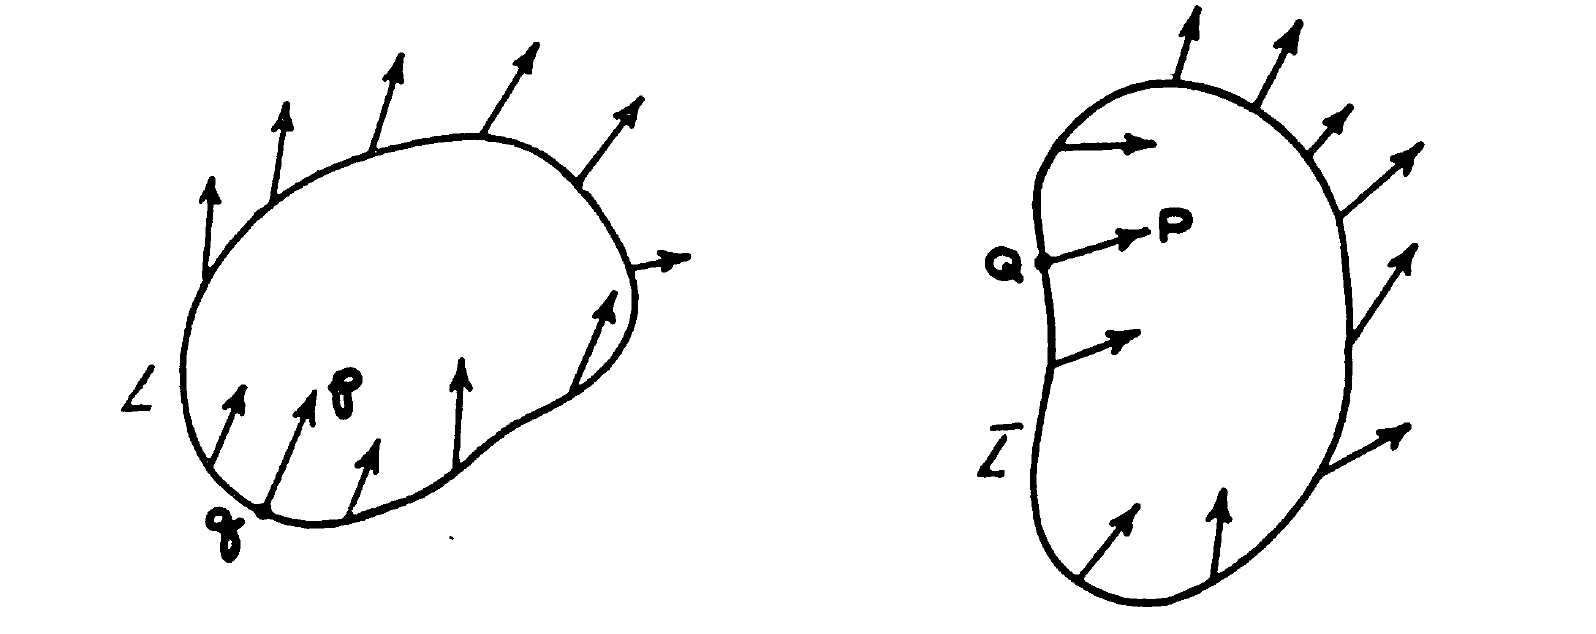
\includegraphics[scale=0.225]{images/circulation}  \end{center}  

\end{frame}

\begin{frame}
     \emph{Für jede geschlossene Kurve im Phasenraum ist}
    \begin{displaymath}
    \Gamma = \oint \sum_{i=1}^{n} p_i d q_i = \oint \sum_{i=1}^{n} P_i d Q_i
    \end{displaymath}
     \emph{eine Invariante gegenüber der kanonischen Transformationen.}
 
\end{frame}
    
    \subsection{Lagrange Klammer}
    \begin{frame}
    \frametitle{Lagrange- und Poisson-Klammer}

    Seien $q_i$ und $p_i$ zwei Koordinatensysteme, $u$ und $v$ Parameter. \\

    \begin{align*}
    \textbf{Lagrange-Klammer: } \qquad    [u,v] = \sum_{i=1}^{n} \left(   \frac{\partial q_i}{\partial u} \frac{\partial p_i}{\partial v} - \frac{\partial q_i}{\partial v} \frac{\partial p_i}{\partial u}  \right)  \\
    \textbf{Poisson-Klammer: } \qquad    (u,v) = \sum_{i=1}^{n} \left(   \frac{\partial u}{\partial q_i} \frac{\partial v}{\partial p_i} - \frac{\partial v}{\partial q_i} \frac{\partial u}{\partial p_i}  \right)  
    \end{align*}

\end{frame}

\begin{frame}
    Es gilt:
    \vspace{5mm}
    \begin{itemize}
        \item Die kanonischen Transformationen sind diejenigen Transformationen von $q_i,p_i$ zu $Q_i,P_i$, für welche die \emph{Lagrange-Klammer} invariant ist.
        \vspace{5mm}
        \item Die kanonischen Transformationen sind diejenigen Transformationen von $q_i,p_i$ zu $Q_i,P_i$, für welche die \emph{Poisson-Klammer} invariant ist.
    \end{itemize}
    
\end{frame}

    
    \subsection{Infinitesimale kanonische Transformationen}
    \begin{frame}
    Zwei kanonische Transformationen:
    \begin{align*}
        \sum_{i=1}^{n} (p_i \delta q_i - P_i \delta Q_i) &= \delta S \\
        \sum_{i=1}^{n} (P_i \delta Q_i - \bar{p}_i \delta \bar{q}_i) &= \delta \bar{S}
    \end{align*}
    
    Summe ist wieder kanonische Transformation:
        \begin{align*}
        \sum_{i=1}^{n} (p_i \delta q_i - \bar{p}_i \delta \bar{q}_i) &= \delta (S + \bar{S}) 
        \end{align*}
        
    Für jedes $S=S(q_1,\ldots,q_n; Q_1,\ldots,Q_n;t),\quad t>0$ gibt es eine Transformation.
    
\end{frame}


\begin{frame}
    \begin{align*}
        t,&\qquad t+\Delta t \\
        Q_k &= q_k + \Delta q_k \\
        P_k &= p_k + \Delta p_k
    \end{align*}
    
    \begin{align*}
        \Longrightarrow \qquad \Delta q_i &= \frac{\partial B}{\partial p_i} \Delta t,\\
                         \Delta p_i &= -\frac{\partial B}{\partial q_i} \Delta t
    \end{align*}
    
    mit
    
    \begin{displaymath}
        B(q_1,\ldots,q_n; p_1,\ldots,p_n;t) = -\frac{\partial S}{\partial t}
    \end{displaymath}
\end{frame}

\begin{frame}
\hspace*{-2.2cm}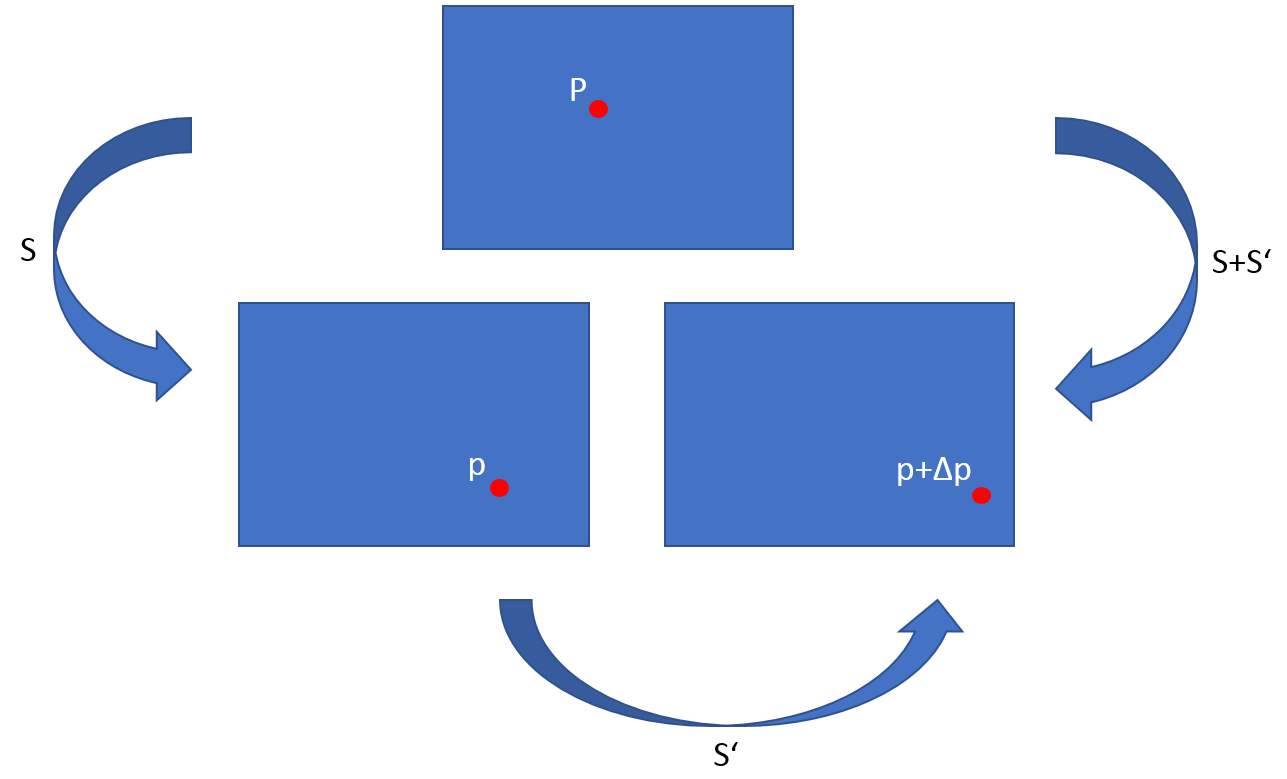
\includegraphics[scale=0.375]{images/ImagTrans}
\end{frame}

\begin{frame}
    \hspace*{-2.2cm}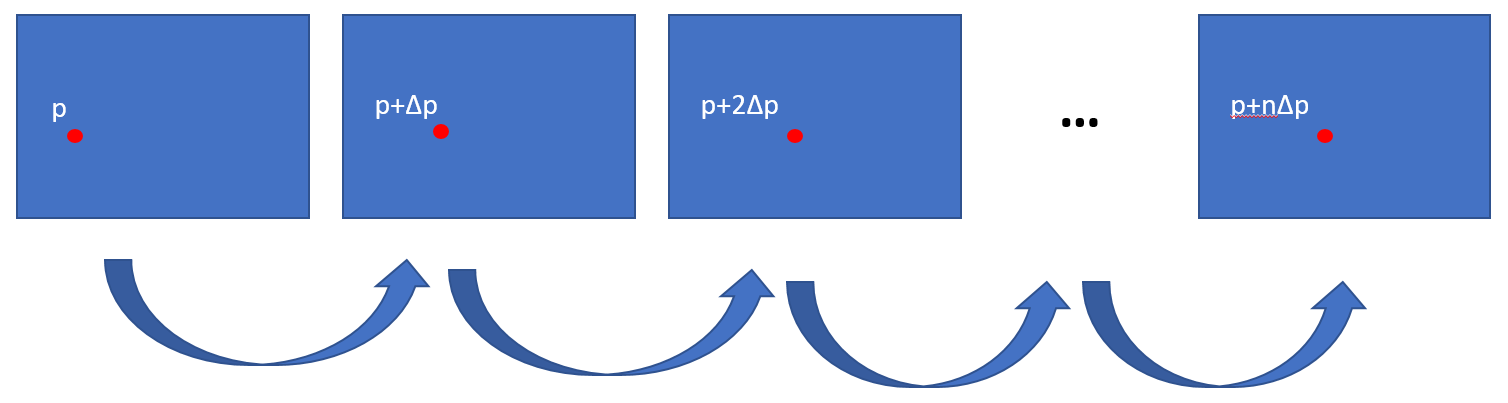
\includegraphics[scale=0.322]{images/TransFlow}
\end{frame}

\begin{frame}
    \begin{align*}
    \Delta q_i &= \frac{\partial B}{\partial p_i} \Delta t,\\
    \Delta p_i &= -\frac{\partial B}{\partial q_i} \Delta t \\[5mm]
      \Delta t &\longrightarrow 0 \\[5mm]
    \frac{dq_i}{dt}  &= \frac{\partial B}{\partial p_i},\\
    \frac{dp_i}{dt} &= -\frac{\partial B}{\partial q_i} 
    \end{align*}
    
    \begin{center} $\rightarrow$ Das sind die kanonischen Bewegungsgleichungen, wobei $B=H$. \end{center}

\end{frame}
        
    \subsection{Das Phasenfluid als kanonische Transformationen}
    \begin{frame}
    \frametitle{Phasenfluid und kanonische Transformation}
    Zu sehen ist also
    \begin{itemize}
        \item Das Phasenfluid wird durch die Hamilton-Gleichungen beschrieben
        \item Zwei Zustände des Phasenfluid können durch kanonische Transformation in Bezug gebracht werden
        \item Für infinitessimal kleine Zustandsübergänge ist die Transformation explizit gegeben
        \item \emph{Die Bewegung des Phasenfluids ist eine stetige Abfolge kanonischer Transformationen}
    \end{itemize}
    
    \begin{displaymath}
        S(q_i,\ldots,q_n;Q_1,\ldots,Q_n;t), \quad t>0
    \end{displaymath}
    
\end{frame}

\begin{frame}
    Bisher:
    \begin{itemize}
        \item Wahl beliebiger generierender Funktion $S$
        \item Damit erhielten wir $B = -H$
    \end{itemize}
    \vspace{1cm}
    Nun Rückwärts:
    \begin{itemize}
        \item Hamilton-Funktion $H$ ist zu physikalischem Problem gegeben
        \item \begin{displaymath} -H = B = \frac{\partial S}{\partial t} \end{displaymath}
        \item Finde $S$
    \end{itemize}
    
\end{frame}


\begin{frame}
    Zu lösen ist also die partielle Differenzialgleichung

    \begin{displaymath}
        \frac{\partial S}{\partial t} + H = 0
    \end{displaymath} \\
        \vspace{1cm}
    $\longrightarrow$ Haben wir damit nicht wieder dasselbe Problem wie zu Beginn? 
\end{frame}

\begin{frame}
    Nicht ganz: \\
            \vspace{1cm}
    Hamilton findet eine Funktion, die diese Gleichung löst und damit ermöglicht, die kanonische Transformation explizit anzugeben:    
    \begin{center} \emph{Die charakteristische Funktion} \end{center}
\end{frame}

\begin{frame}
    \begin{align*}
        \text{Prinzip d. kl. Wirkung: } \quad A &= 2 \int_{\tau_1}^{\tau_2} T~dt \\
         &=  \int_{\tau_1}^{\tau_2} \sum_{i=1}^{n} p_i \dot{q}_i ~dt \\
         &= \int_{\tau_1}^{\tau_2} \sum_{i=1}^{n} p_i ~ dq_i \\[5mm]
        \text{Energieerhaltung: } \quad  H&(q_1,\ldots,q_n,p_1,\ldots,p_n) - E = 0 \\[5mm]
      \Leftrightarrow  \text{Jacobi: } \quad \min A ~ \text{ mit } ~ A &= \sqrt{2} \int_{\tau_1}^{\tau_2} \sqrt{E-V} ~ d\bar{s}
    \end{align*}
\end{frame}

\begin{frame}
  \vspace*{-0.75cm} \hspace*{-2.3cm} 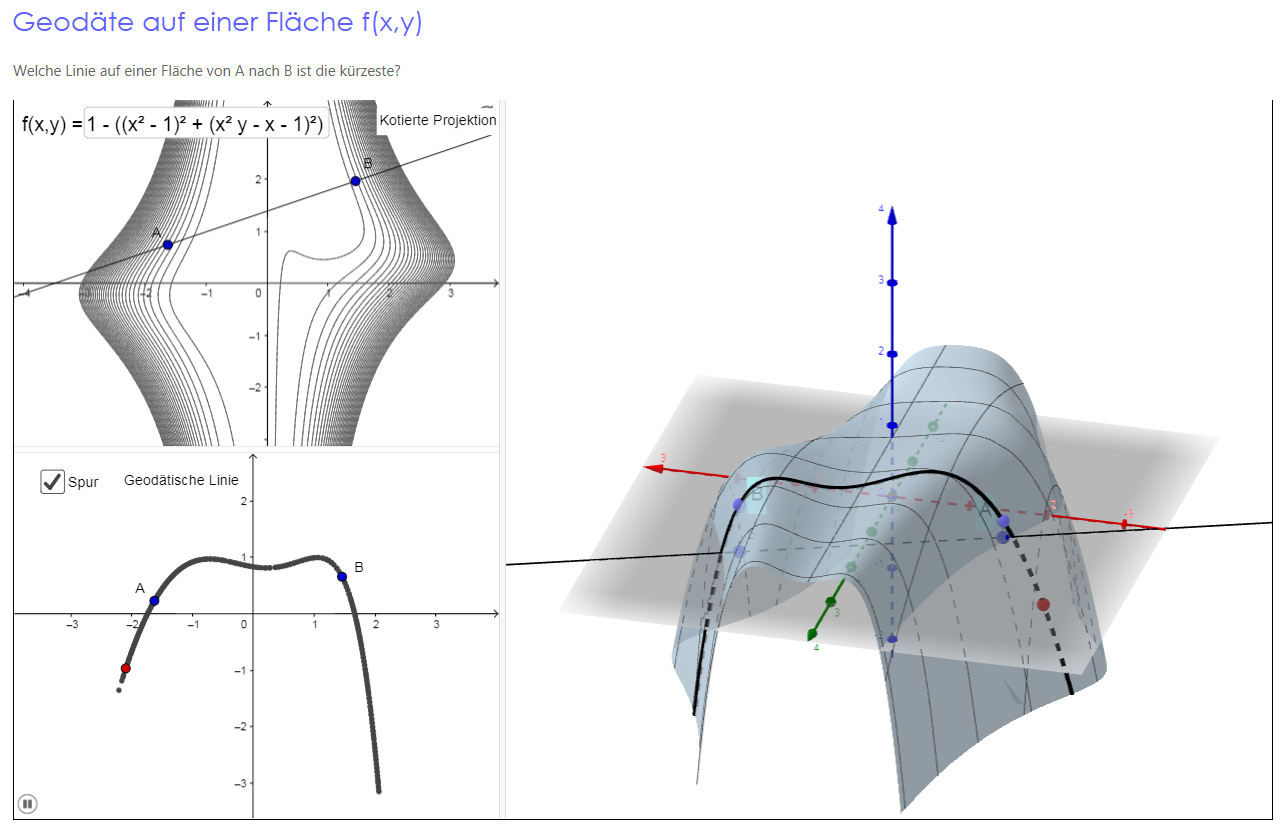
\includegraphics[scale=0.4]{images/geodaete}
\end{frame}

\begin{frame}
    \begin{itemize}
        \item Hamiltons charakteristische Funktion liefert die Länge der Geodäte zwischen Anfangs- und Endpunkt auf einer Energie-Fläche im Phasenraum
        \item Hamiltons charakteristische Funktion ist die generierende Funktion für die zugehörige kanonische Transformation
        \item Die mit Hamiltons charakteristischer Funktion generierte kanonische Transformation beschreibt die Bewegung eines Partikels im Phasenfluid
        \item $S(q_i,\ldots,q_n;Q_1,\ldots,Q_n;t)$ liefert für Anfangspunkte $Q_1,\ldots,Q_n$ für jedes $t>0$ die Lösungen $q_i(t),\ldots,q_n(t)$ der kanonischen Gleichungen 
     \end{itemize}
\end{frame}
        
\section{Die Hamilton-Jacobi-Gleichung}

    \subsection{Jacobis Transformationstheorie}
    
    \subsection{Lösung durch Separation}
    
    \subsection{Partielle Differenzialgleichungen bei Hamilton und Jacobi}

    \subsection{Geometrische Lösung und Wellenanalogie}

\section{Zusammenfassung}


\end{document}